\chapter{AI 伦理、版权与科研规范}

\section{案例目标}

第 35 章讨论的是：当 AI 帮你写出一段科研代码时，怎样通过验证回路判断它值不值得留下。第 36 章讨论的是：当 AI 开始分步骤调用工具时，怎样用 gate、停止条件和人工接管保护工作流。第 37 章则把同样的思路带到了论文阅读、claim ledger 和报告写作里。

本章继续沿着这条主线往前走，但讨论的是一个更容易被误解成“口号”的问题：\textbf{当 AI 已经进入科研项目时，伦理、版权、学术诚信和使用声明到底怎样落到日常 workflow 里？}

本章的目标有三点：

\begin{enumerate}
    \item 理解 AI 伦理与科研规范不是抽象态度表态，而是一组可以写进 notebook、项目记录和课程要求的具体边界；
    \item 学会把 AI 使用场景区分成“允许但要披露”“要先做版权 / 许可检查”“必须保持人工签字权”和“当前不该做”四类出口；
    \item 学会从一份结构化的 usage log 出发，写出更诚实、可检查的 AI-use statement，而不是事后凭印象补一句“使用过 AI”。
\end{enumerate}

\section{为什么这一章紧跟在第 35 章到第 37 章之后}

如果说第 35 章强调的是“AI 生成代码之后要验证”，第 36 章强调的是“AI 执行多步骤流程时要有边界”，第 37 章强调的是“AI 阅读文献时要保留 claim 与出处”，那么本章要强调的就是：\textbf{这些边界最后都要落到项目规范层。}

学生在真实课程和科研里最容易遇到的，不是“应不应该完全禁用 AI”，而是下面这些更具体的问题：

\begin{itemize}
    \item 我能不能让 AI 帮我整理自己的观察笔记？
    \item 我能不能把未发表数据贴进第三方聊天工具？
    \item 我能不能让 AI 重写一段论文原文，再直接放进报告？
    \item 我能不能让 AI 决定最终科学结论够不够强？
    \item 我在作业或项目报告里到底该怎样披露 AI 的参与方式？
\end{itemize}

如果这些问题没有被拆成清楚的 workflow，学生很容易退回到两个都不好的极端：

\begin{itemize}
    \item 要么把“AI 伦理”理解成抽象说教，最后不知道实际该怎么做；
    \item 要么只看省时程度，什么地方都让 AI 先上，再事后补救。
\end{itemize}

所以本章的核心立场是：\textbf{科研规范不是写在海报上的道德标语，而是你怎样处理材料来源、共享边界、引用、许可、最终签字权和使用声明。}

\section{一个极小的 AI 使用场景卡片数据集}

配套 notebook 使用 \nolinkurl{ai_ethics_workflow_demo.csv}。这不是法律条文汇编，也不是在线政策数据库，而是一组完全本地、教学用途的\textbf{AI 使用场景卡片}。每一行代表一个学生在课程项目或科研小项目里可能真的会遇到的 AI 使用请求，包含：

\begin{itemize}
    \item \texttt{case\_id}；
    \item \texttt{workflow\_stage}；
    \item \texttt{speed\_gain\_score}；
    \item \texttt{ai\_use\_type}；
    \item \texttt{source\_material}；
    \item \texttt{sharing\_boundary}；
    \item \texttt{claim\_verification}；
    \item \texttt{reference\_route}；
    \item \texttt{disclosure\_required}；
    \item \texttt{scenario\_text}。
\end{itemize}

这里的设计非常刻意。数据里既有明显适合保留的使用方式，也有几类最容易让学生在“省时间”的名义下越界的场景：

\begin{itemize}
    \item 让 AI 编造自己还没读过的 related-work 引用；
    \item 把未发表、共享边界不清楚的数据贴进第三方服务；
    \item 让 AI 改写受版权保护的论文原文；
    \item 让 AI 代替你做最终 scientific signoff；
    \item 以及几类其实很常见、也可以保留的低风险辅助任务，例如整理自己的笔记、重构自己的 notebook、润色已核实的使用声明。
\end{itemize}

因此，本章真正要训练的不是“怎样背伦理原则”，而是更具体的能力：

\begin{itemize}
    \item 你能不能把 AI 用途和材料边界一起看，而不是只看速度收益？
    \item 你能不能区分“要披露”“要许可检查”“必须人工决定”和“现在就不该做”这几种不同状态？
\end{itemize}

\section{先看一个很常见的 baseline：只按省时程度挑 AI 用法}

如果没有结构化规范，一个很常见的 baseline 就是：\textbf{按 \texttt{speed\_gain\_score} 从高到低排序，优先把最省时间的任务交给 AI。}

\begin{examplebox}[只看省时程度的 baseline]
\begin{lstlisting}[style=pythonstyle]
top_cases = sorted(rows, key=lambda row: row["speed_gain_score"], reverse=True)[:4]
\end{lstlisting}
\end{examplebox}

这种做法的问题非常直接：它把“省时”误当成“适合自动化”，却没有先问：

\begin{itemize}
    \item 这份材料能不能被发送给外部服务？
    \item 这段文本或图像是否涉及版权与复用许可？
    \item 这里要求的是语言整理，还是最终 scientific signoff？
    \item 这件事最后是否应该被写进 AI-use statement？
\end{itemize}

在本章教学数据上，按省时程度排名前四的案例里会混入：

\begin{itemize}
    \item 一个“让 AI 猜还没读过的引用”的场景；
    \item 一个“上传未发表数据到共享边界不清楚的服务”的场景；
    \item 一个“改写受版权保护论文文字”的场景；
    \item 只有一个是真正适合直接保留并披露的低风险案例。
\end{itemize}

因此 notebook 中会得到表~\ref{tab:ch38_baseline_vs_policy} 这个最小对照：

\begin{table}[htbp]
\centering
\small
\setlength{\tabcolsep}{4pt}
\begin{tabular}{@{}p{0.22\textwidth}>{\centering\arraybackslash}p{0.16\textwidth}>{\centering\arraybackslash}p{0.16\textwidth}>{\centering\arraybackslash}p{0.16\textwidth}p{0.20\textwidth}@{}}
\toprule
方法 & 可直接披露比例 & 允许案例覆盖率 & 被拦截案例混入率 & 教学解读 \\
\midrule
省时优先前四项 & 0.25 & 0.20 & 0.75 & 高风险案例容易因为“看起来省事”被排到前面 \\
结构化规范 workflow & 1.00 & 1.00 & 0.00 & 先检查边界，再决定哪些用途可以留下并披露 \\
\bottomrule
\end{tabular}
\caption{本章 notebook 中两个最小流程的对照。重点不是“谁更会用 AI”，而是谁更尊重材料、权限和签字边界。}
\label{tab:ch38_baseline_vs_policy}
\end{table}

\section{规范 workflow 的关键不是“讲道理”，而是“先 route 再使用”}

本章 notebook 把 AI 使用场景拆成四类非常具体的出口：

\begin{itemize}
    \item \textbf{allow with disclosure}：低风险、可保留的辅助使用，但必须如实披露；
    \item \textbf{license review}：先做版权、引用、复用许可或 quotation boundary 检查；
    \item \textbf{human only}：最终 scientific signoff 仍然必须由人承担；
    \item \textbf{prohibit}：当前不该做，例如编造引用、上传共享边界不清的数据。
\end{itemize}

最小 routing 逻辑可以写成：

\begin{examplebox}[一个最小规范路由逻辑]
\begin{lstlisting}[style=pythonstyle]
if ai_use_type == "invent_missing_citation":
    prohibit
elif source_material == "proprietary_data":
    prohibit
elif sharing_boundary == "external_unknown":
    prohibit
elif source_material in {"copyrighted_text", "published_figure"}:
    license_review
elif claim_verification == "final_signoff":
    human_only
else:
    allow_with_disclosure
\end{lstlisting}
\end{examplebox}

这里最重要的，不是背住 route 名字本身，而是学会问一组更基础的问题：

\begin{itemize}
    \item 我现在处理的是自己的材料、公开材料，还是受限制材料？
    \item 我把它发给的工具，保存和训练边界清不清楚？
    \item 这一步是在组织语言，还是在替我承担最终判断？
    \item 这件事如果真的做了，能不能诚实地写进使用声明？
\end{itemize}

图~\ref{fig:ch38_policy_pipeline} 给出了本章 notebook 中的最小规范流程。

\begin{figure}[htbp]
\centering
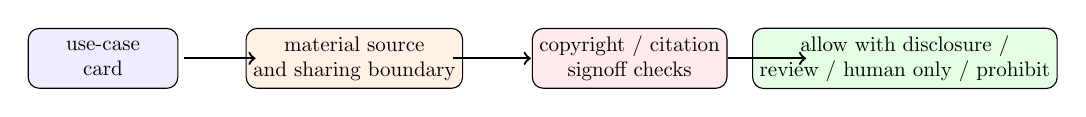
\begin{tikzpicture}[every node/.style={align=center}, scale=0.76, transform shape]
\node[draw, rounded corners, fill=blue!7, minimum width=2.5cm, minimum height=1.0cm] at (0,0) (card) {use-case\\card};
\node[draw, rounded corners, fill=orange!10, minimum width=3.2cm, minimum height=1.0cm] at (4.2,0) (material) {material source\\and sharing boundary};
\node[draw, rounded corners, fill=red!8, minimum width=3.1cm, minimum height=1.0cm] at (8.8,0) (review) {copyright / citation\\signoff checks};
\node[draw, rounded corners, fill=green!10, minimum width=3.2cm, minimum height=1.0cm] at (13.4,0) (route) {allow with disclosure /\\review / human only / prohibit};

\draw[->, thick] (1.35,0) -- (2.55,0);
\draw[->, thick] (5.85,0) -- (7.15,0);
\draw[->, thick] (10.45,0) -- (11.75,0);
\end{tikzpicture}
\caption{本章 notebook 中的最小科研规范流程。先判定材料与边界，再决定 AI 是否可以进入下一步。}
\label{fig:ch38_policy_pipeline}
\end{figure}

\section{披露、许可和最终签字权是三条不同边界}

学生最容易混淆的一点，是把下面三件事混成一句“只要说明用了 AI 就行”：

\begin{enumerate}
    \item \textbf{披露（disclosure）}：你是否诚实说明 AI 在项目里做了什么；
    \item \textbf{许可（permission / license）}：你是否有权重用某段文字、某张图或某份材料；
    \item \textbf{最终签字权（final signoff）}：最后哪些判断必须由人自己承担责任。
\end{enumerate}

这三者并不等价：

\begin{itemize}
    \item 你可以诚实披露一件事，但那件事本身仍然不该做，例如上传共享边界不清楚的未发表数据；
    \item 你可以引用一篇论文，但并不自动意味着可以把它的文字或图像交给 AI 任意改写后再重用；
    \item 你可以让 AI 帮你组织语言，但不应该让它替你决定最终 scientific claim 是否成立。
\end{itemize}

也就是说，\textbf{披露不是免责条款，许可不是格式细节，最终签字权也不能被“AI 帮忙”悄悄转移。}

\section{先有 usage log，再写 AI-use statement}

很多学生在项目快结束时，才开始想“我要不要在报告里写一句用了 AI”。这时最常见的问题是：

\begin{itemize}
    \item 只记得大概用过，却记不清具体在哪几步；
    \item 把“语言润色”和“决定结论”混成同一类；
    \item 只写了一句泛泛而谈的话，既不能帮助读者理解，也不能保护自己。
\end{itemize}

更可靠的顺序其实相反：

\begin{enumerate}
    \item 先记录 use-case card；
    \item 再对每个案例做 route；
    \item 再保留允许使用、待许可检查、人工保留和禁止项的队列；
    \item 最后才根据真实留下来的使用记录，生成 AI-use statement。
\end{enumerate}

在本章 notebook 里，最终 statement skeleton 并不是“AI 很强，所以帮了很多”，而是更具体的东西，例如：

\begin{itemize}
    \item AI 只用于整理作者自己的笔记、重构作者自己的 notebook、总结公开文档和润色已核实的说明；
    \item 所有最终科学结论、引用、权限检查和发布决策仍由作者本人完成；
    \item 未发表数据没有被发送到共享边界不清楚的外部服务；
    \item 没有保留任何未阅读、未核实的 AI 猜测引用。
\end{itemize}

这类 statement 的价值，不在于显得“规范”，而在于它能被你自己的 workflow 记录支撑。

\section{一个更适合科研规范审查的 prompt 结构}

如果任务已经进入 AI 使用规范，prompt 也不应该只是“帮我写个伦理声明”。更好的做法是把\textbf{材料来源、共享边界、最终签字权和输出格式}一起说清楚。例如：

\begin{examplebox}[一个更适合科研规范审查的 prompt 模板]
\begin{lstlisting}[style=pythonstyle]
prompt = """
你是我的科研规范助手。

任务：
1. 先阅读 use-case table，而不是先给口号；
2. 把每个案例 route 到 allow with disclosure、
   license review、human only 或 prohibit；
3. 标出哪些事项必须保留 human ownership；
4. 只有在 route 完整后，才起草 AI-use statement。

输出格式：
- Allowed uses with disclosure
- License review queue
- Human-only decisions
- Prohibited uses
- Draft AI-use statement
"""
\end{lstlisting}
\end{examplebox}

这里真正起作用的，不是什么神秘的提示词技巧，而是你有没有先要求 AI 保留\textbf{规范结构}。如果这个结构一开始就没有建立好，最后那段“声明”通常只会变成好听但空泛的表态。

\section{配套 notebook 做了什么}

本章 notebook 采用的是一个 teaching-first 的最小设计：

\begin{itemize}
    \item 先读取 use-case 表，并打印 workflow stage、材料类型与参考 route 统计；
    \item 用只看 \texttt{speed\_gain\_score} 的方式做一个 naive automation baseline；
    \item 再实现一个最小 policy routing workflow；
    \item 输出 allow、license review、human only 和 prohibit 四个队列；
    \item 最后生成 prompt 模板、workflow checklist、AI-use statement skeleton 和 ethics snapshot。
\end{itemize}

这份 notebook 不追求真实校规接口，也不连接外部政策服务。它真正要教的是：\textbf{把 AI 伦理、版权和科研规范翻译成一个学生自己能执行的本地工作流。}

\section{和 Capstone 项目的关系}

到这里为止，Part V 已经不只是在讲“模型”，而是在讲\textbf{现代 AI 进入科研项目之后，学生怎样维持可信工作流}：

\begin{itemize}
    \item 第 35 章讲代码验证；
    \item 第 36 章讲多步骤代理的工具边界；
    \item 第 37 章讲论文阅读与报告写作中的证据边界；
    \item 本章讲 AI 使用边界、版权、许可与使用声明。
\end{itemize}

到了 Capstone 项目里，这些内容几乎一定会重新出现。学生不仅要会“用 AI”，还要会：

\begin{itemize}
    \item 说明哪些地方用了 AI；
    \item 说明 AI 处理的是谁的材料、在哪个边界里处理；
    \item 保留最终 scientific signoff；
    \item 在报告中写出诚实、具体、可检查的 AI-use statement。
\end{itemize}

如果一个项目只写“本项目使用了 AI 辅助”，其实几乎没有提供可检查信息。真正有价值的，是它能不能回答：

\begin{itemize}
    \item AI 具体辅助了哪一步；
    \item 哪些内容是 AI 没有被允许决定的；
    \item 哪些材料根本没有被发送给外部服务；
    \item 哪些文字、图像和引用最终由作者自己核查并承担责任。
\end{itemize}

\begin{warnbox}[AI 伦理与科研规范中的常见误区]
\begin{itemize}
    \item 只要说“我用了 AI”，就以为已经完成全部规范要求；
    \item 把“省时间”当成“适合自动化”的充分理由；
    \item 让 AI 猜自己还没读过的引用；
    \item 把未发表或共享边界不清楚的数据发给第三方服务；
    \item 把最终 scientific signoff 伪装成“只是帮我参考一下”。
\end{itemize}
\end{warnbox}

\section{AI 助手如何帮助你}

在这个案例里，AI 助手最适合帮助你：

\begin{itemize}
    \item 把分散的 use-case 记录整理成更清楚的 usage log；
    \item 帮你区分语言润色、材料复用、引用生成和最终签字权这些不同任务；
    \item 把允许保留的使用方式整理成更自然的 AI-use statement 草稿；
    \item 把待许可检查项改写成一份更清楚的人工核查清单；
    \item 帮你把课程要求翻译成项目级 checklist。
\end{itemize}

但最终哪些材料可以被共享、哪些内容涉及版权与许可、哪些 claim 可以署名提交，以及哪些 AI 使用必须被明确披露，仍然必须由你自己判断并承担责任。

\section{练习}

\begin{exercisebox}[基础练习]
把教学数据里一条原本允许披露的案例改成“共享边界不清楚的外部服务”场景，也就是把 \texttt{sharing\_boundary} 改成 \texttt{external\_unknown}。重新运行 notebook，观察它为什么会被 route 到 \texttt{prohibit}。
\end{exercisebox}

\begin{exercisebox}[进阶练习]
请再添加一条“AI 帮你生成报告封面配图”的 use-case card，并明确写出：素材来源、是否涉及版权、是否需要 disclosure、以及它应当进入哪一个 route。
\end{exercisebox}

\begin{exercisebox}[开放练习]
结合你自己的课程项目，设计一个最小 AI-use statement 模板。至少包含：AI 参与的步骤、材料边界、未交给 AI 的关键判断，以及一条你愿意公开签字负责的核查说明。
\end{exercisebox}

\section{本章小结}

本章并不试图把复杂的法律、校规或期刊政策压缩成几条万能口号，而是强调一个更可执行的思路：\textbf{把 AI 伦理、版权和科研规范翻译成 use-case、route、queue 和 usage statement。}

只要你能把“材料来源是什么、共享边界在哪里、最终谁来签字、哪些内容必须披露”这几件事持续写进 workflow，那么 AI 就更可能成为一个可管理的科研工具，而不是一个让责任边界越来越模糊的捷径。
